\chapter{Introduction}
\label{chpt:introduction}

% Accurate chromosome segregation during cell division requires that the sister kinetochores on each replicated chromosome are stably attached to microtubules emanating from opposite spindle poles before the cell divides. If one or more kinetochores fail to attach to microtubules, they activate a biochemical signaling cascade known as the spindle assembly checkpoint (SAC). This cascade produces an anaphase-inhibitory signal known as the ‘‘mitotic checkpoint complex’’ (MCC). MCC inhibits the anaphase promoting complex/cyclosome (APC/C) to prevent the cell from transitioning from prometaphase to anaphase, thus avoiding chromosome mis-segregation.

% How the SAC blocks the progression of mitosis in the presence of a single unattached kinetochore and releases the block promptly once all attachment is secured remains unclear. Here, I summarize our discovery that the SAC, like many other biochemical switches, exploits cooperativity to achieve such sensitivity. Furthermore, I look into potential molecular mechanisms of this cooperativity.

\section{Mitosis, spindle, and the kinetochore-spindle microtubule attachment in human cells}

\begin{figure}
    \centering
    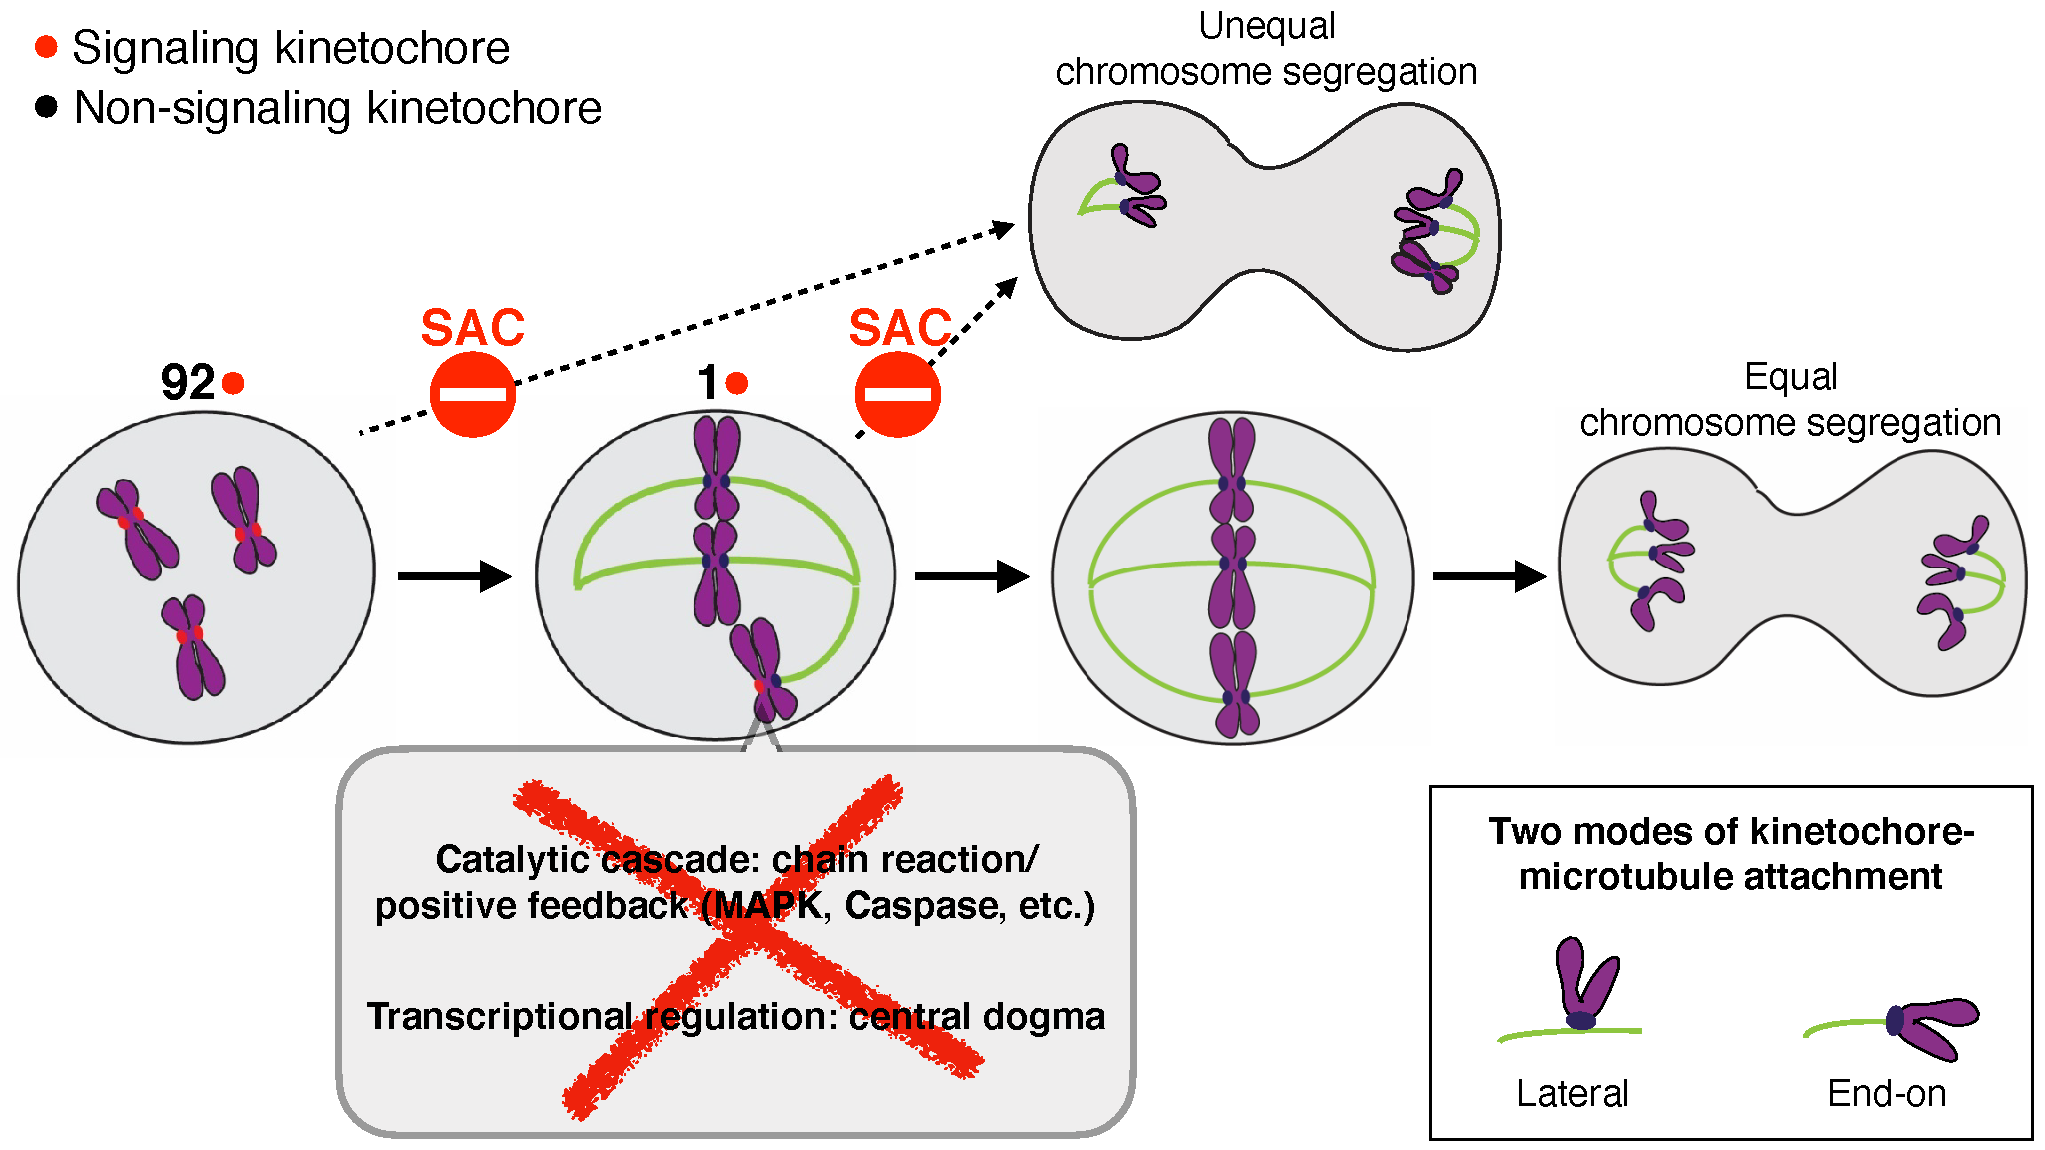
\includegraphics[width=0.9\textwidth]{chapters/figures/SACRole.pdf}
    \caption{\textbf{The gradual establishment of kinetochore-spindle microtubule attachment and the role of the SAC in ensuring equal chromosome segregation.}}
    \noindent\justifying Kinetochores without end-on microtubule attachment activate the spindle assembly checkpoint (SAC) to prevent premature anaphase onset. The sensitivity of the SAC is unlikely to be facilitated by an enzymatic amplification cascade, given our current understanding of the biochemical pathway of the SAC \cite{InhibitorUltrasensitivity, Caspase}. Transcriptional regulations that amplify signals via the central dogma and potential oligomerization of the involved transcriptional factors \cite{TFMultimerization} are also unlikely because the genome is highly condensed in the chromosome during the prometaphase.
    \label{SACRole}
\end{figure}

\section{The spindle assembly checkpoint (SAC) signaling in human cells: the core pathway and the corona pathway}

Cells deploy the spindle assembly checkpoint (SAC) to monitor the progress of the establishment of the kinetochore-microtubule attachment. The SAC is activated at kinetochores without end-on microtubule attachment to block premature anaphase onset \cite{GSK923295MonastrolCotreatment, GSK923295LateralAttachmentEM, LateralAttachmentSAC}. This block allows time for the establishment of the end-on kinetochore-microtubule attachment. Once all attachment is secured, the SAC is silenced and the block is lifted \cite{SACActivationAndSilencing}. Mitosis is then resumed, leading to equal segregation of chromosomes into daughter cells (see \myref{SACRole}).

The SAC can be activated by a single unattached kinetochore, and the strength of the signaling activity is positively correlated with the number of signaling kinetochores in mammalian cells \cite{RiederNormalProgression, Rheostat, Ablation}. The SAC in mammalian cells relies on the kinetochore-localized signaling scaffold \protein{Knl1} as well as the corona \cite{GSK923295LateralAttachmentEM, LateralAttachmentSAC, CoronaActivatesSAC}. We refer to them as the core pathway (which will be the main focus of my thesis; see \myref{CoreSAC}) and the corona pathway, respectively \cite{100nMNoc, eSAC}.

\begin{figure}
    \centering
    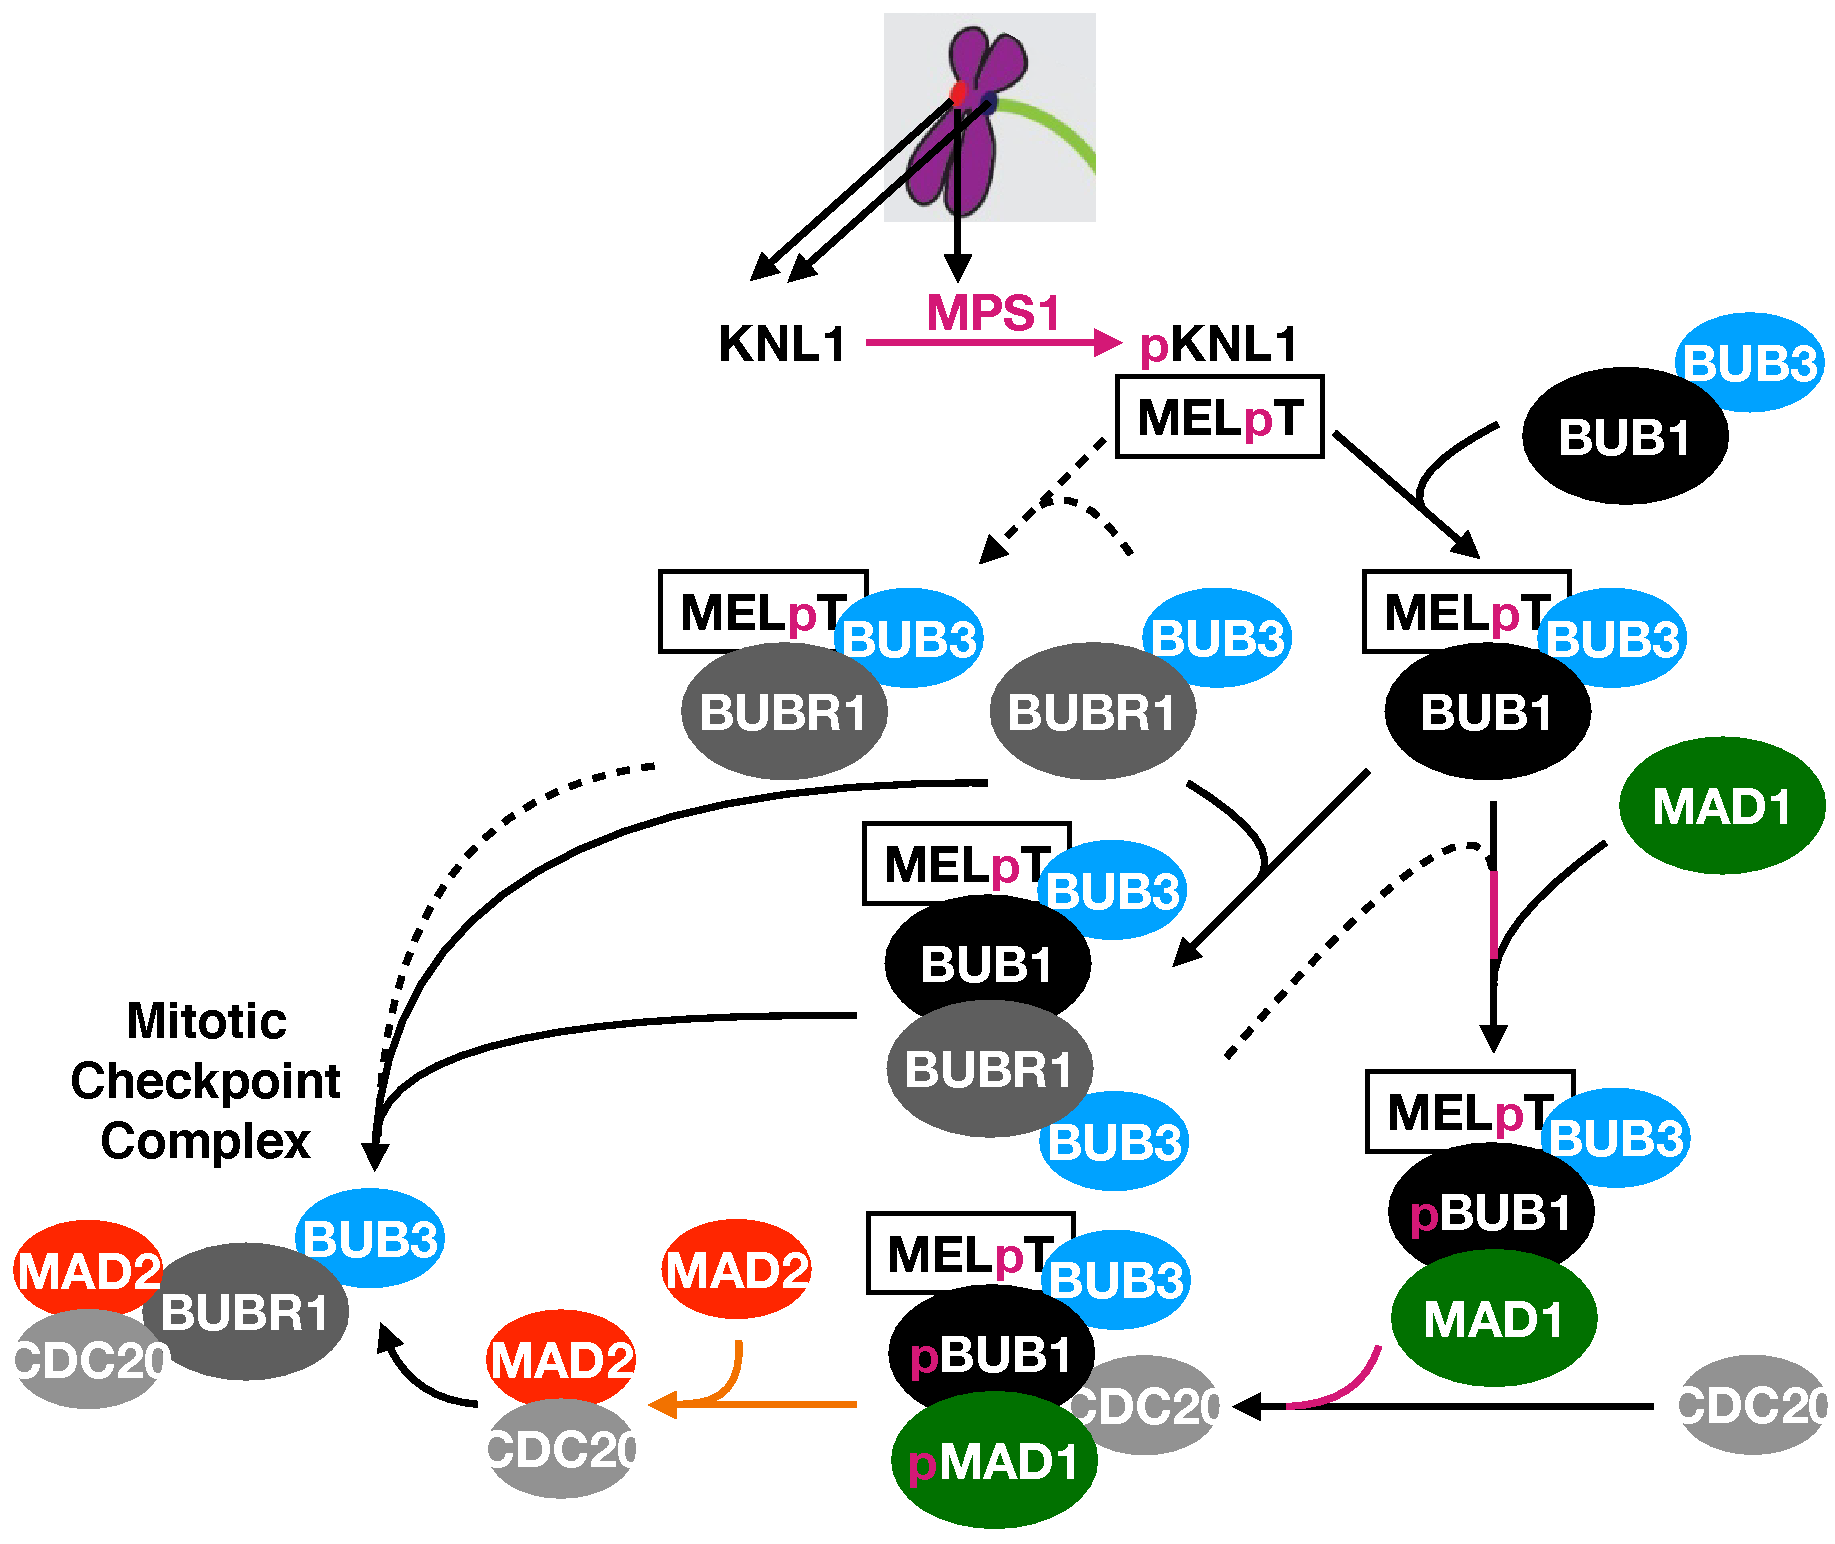
\includegraphics[width=0.94\textwidth]{chapters/figures/CoreSAC.pdf}
    \caption{\textbf{The biochemical interactions and reactions of the core SAC signaling pathway.}}
    \noindent\justifying In the core SAC signaling pathway, signaling kinetochores recruit the kinase \protein{Mps1} which phosphorylates the consensus MELT motifs on the scaffold protein \protein{Knl1}. Phosphorylated MELT motifs (the ``MELpT'' rectangle in the figure) will then recruit a series of SAC proteins and eventually generate the effector molecule known as the Mitotic Checkpoint Complex (MCC), which blocks the progression of mitosis. \protein{Cdc20} binds to signaling kinetochores cooperatively via its interactions with \protein{Bub1} and \protein{Mad1} \cite{BUB1-CDC20-MAD1, Tripartite}. Black solid arrows indicate direct binding or participation, which is either the consensus understanding in the field \cite{MPS1Localization_Ji, MPS1Localization_Hiruma, RecombinantKNL1, MELTActivity, BubBiochem, BubR1TwoPools, BUB1CD1-MAD1CStructure, Faesen2017, BUB1-CDC20-MAD1, Tripartite} or experimentally proved in my thesis research (see \myref{per_se}). Black dashed arrows indicate arguable \cite{BubBiochem, BubR1TwoPools} or hypothetical direct binding or participation. Magenta arrows and texts indicate \protein{Mps1} or involvement of \protein{Mps1}-mediated phosphorylation \cite{Ji2017eLife}. The orange arrow indicate catalytic reactions leading to the formation of the \protein{Cdc20}-\protein{Mad2} dimer, which will be the focus of \myref{chpt:4}. The green \protein{Mad1} oval indicates the \protein{Mad1}-\protein{Mad2} heterotetramer (see \myref{chpt:4}). This heterotetramer is extremely stable in the budding yeast \cite{StableHeterotetramer}. The molecular weight of \protein{Mad1} (an extended protein mainly composed of \textalpha{}-helices according to the prediction of AlphaFold \cite{AlphaFold}) is also much greater than the molecular weight of \protein{Mad2} (a globular protein \cite{Structure1GO4}). Therefore, the \protein{Mad1}-\protein{Mad2} heterotetramer is also sometimes simply referred to as ``\protein{Mad1}'' in the following context.
    \label{CoreSAC}
\end{figure}

\protein{Knl1} possesses multiple consensus MELT motifs \cite{MELTEvolution}, which are phosphorylated at signaling kinetochores \cite{MPS1-KNL1_London2012, MPS1-KNL1_Shepperd2012, MPS1-KNL1_Yamagishi2012, MPS1Localization_Ji, MPS1Localization_Hiruma}. Phosphorylated MELT motifs initiate the core SAC signaling pathway by recruiting SAC proteins like \protein{Bub3}, \protein{Bub1}, \protein{BubR1}, \protein{Cdc20}, and the \protein{Mad1}-\protein{Mad2} heterotetramer, thereby promoting the assembly of the mitotic checkpoint complex (MCC) consisting of \protein{BubR1}/\protein{BubR1}-\protein{Bub3} and \protein{Cdc20}-\protein{Mad2} \cite{RecombinantKNL1, MELTActivity, BubBiochem, BubR1TwoPools, BUB1CD1-MAD1CStructure, Faesen2017, BUB1-CDC20-MAD1, Tripartite, SpMCC}. The mitotic checkpoint complex inhibits the E3 ubiquitin ligase anaphase-promoting complex/cyclosome (APC/C) \cite{APC-MCC_Alfieri2016, APC-MCC_Yamaguchi2016}. APC/C ubiquitinates Cyclin B1, a key mitosis regulator, thereby targeting it for proteasome-mediated degradation \cite{CyclinB1Degradation_Clute+Pines1999, CyclinB1Degradation_Chang2003, SeparaseStructure}. Through the inhibition of the APC/C, the degradation of Cyclin B1 is suppressed and the onset of anaphase is delayed.

In the corona pathway of the SAC signaling, the corona recruits the \protein{Mad1}-\protein{Mad2} heterotetramer to signaling kinetochores and promotes the SAC signaling activity \cite{CoronaActivatesSAC}. It should be noted that the core pathway and the corona pathway are not independent in human cells. Corona constituents \protein{Cenp-E} and \protein{Cenp-F} interact with \protein{BubR1} and \protein{Bub1}, respectively \cite{CENPELocalization-BUBR1, CENP-FLimitsStripping}. It has also been suggested that the recruitment of \protein{Mad1} to signaling kinetochores may be cooperative, facilitated by both the corona and \protein{Bub1} \cite{MIS12-CEP57-MAD1-MAD2, siROD_Zhang2019}. We conceptually separate the two pathways because the corona does not exist in the budding yeast, while the core pathway is conserved from yeast to human \cite{YeastNoRZZ}.

\section{MELT motifs and their arrangement in human \protein{Knl1}}

% Alternative splicing is common in intrinsically disordered regions mediating protein-protein interactions \cite{DisorderedRegionsAlternativeSplicing}. However, in many mammals, all of Knl1's MELT motifs within a single exon which is one of the longest internal exons in these mammals (\myref{ExonLength}). No alternatively splicing has been recorded for this region. The splicing machinery has to deploy specific mechanisms to splice long exons like this correctly \cite{InternalExon}.

\begin{table}[H]
    \renewcommand{\arraystretch}{1.5}
    \caption{\textbf{The exon encoding all MELT motifs in \protein{Knl1} ranks among the top 0.03\% by length among all curated internal exons in human and mouse.}}
    \noindent\justifying All putative MELT motifs identified in \cite{MELTEvolution} reside within a single exon and all recorded alternative splice variants of \protein{Knl1} contain this exon in listed mammals. Coordinates of exons (of mouse and human) in the CCDS Database \cite{CCDS} were accessed on May 21, 2020. Exons from coding sequences with either a ``Public'' or a ``Reviewed, update pending'' status were pooled. Redundant entries were removed (because various coding sequences may share a common exon) and the ranking of the MELT motif-encompassing exon was calculated. Due to the lack of data for untranslated regions, only internal exons were included in the analysis. It should be noted that the maximum length of an exon is restricted by the length of the respective protein, and \protein{KNL1} is a long protein of \SI{2342}{} amino acids (the canonical isoform). In a non-canonical isoform of human \protein{Knl1}, this MELT motif-encompassing exon is 166 bases shorter, but still includes all 19 putative MELT motifs.
    \label{ExonLength}
    \begin{center}
        \begin{tabular}{c c c}
            \hline
            Species & Exon length (bases) & Ranking among all curated internal exons\\
            \hline
            Human & 5001 & $99.973\%$\\
            Mouse & 4497 & $99.975\%$\\
            Rat & 3439 & N/A\\
            Cattle & 4020 & N/A\\
            Elephant & 4023 & N/A\\ % What kind of elephant?
            Giant panda & 4017 & N/A\\
            Dog & 3837 & N/A\\
            Bonobo & 3927 & N/A\\
            \hline
        \end{tabular}
    \end{center}
\end{table}

\section{The sensitivity and responsiveness of the SAC}

% Just like one will not completely understand how a machine works just by knowing all the gears involved, we cannot claim to have completely comprehended how the SAC works by just knowing all associated biochemical reactions individually.
% the sensitivity of the SAC
% responsiveness (releasing the block promptly once all attachment is secured)
% How the number of signaling kinetochores changes the strength of the signaling output is not fully understood. This knowledge will help us comprehend how the SAC prevents premature anaphase onset in the presence of a decreasing number of signaling kinetochores from the nuclear envelope breakdown to the metaphase during normal mitotic progression.

\section{Cooperativity is one way to realize ultrasensitivity}

Originally, ``cooperativity'' was used to described the binding of oxygen molecules to the multi-subunit hemoglobin \cite{KNF, MWC}. Cooperativity may amplify the signal or at least sensitize the output by reducing the dampening effect of any changes in the input \cite{CooperativityQA}. To explain such dampening effect, suppose that the output $f(x) \geq 0$ is a monotonically increasing and strictly concave function of the input $x$ for all $x \geq 0$ (like the Langmuir adsorption equation or the Michaelis-Menten kinetics) and that the output is 0 if and only if the input is 0. Comparing the outputs [$f(x_2)$ and $f(x_1)$] corresponding to the inputs ($x_2 > x_1 > 0$), we have

\begin{equation*}
    1 < \dfrac{f(x_2)}{f(x_1)} = \dfrac{f(x_2)}{f[\dfrac{x_1}{x_2} \cdot x_2 + (1-\dfrac{x_1}{x_2}) \cdot 0]} < \dfrac{f(x_2)}{\dfrac{x_1}{x_2}f(x_2) + (1-\dfrac{x_1}{x_2})f(0)} = \dfrac{x_2}{x_1},
\end{equation*}

\noindent which states that the contrast between the outputs is less than the contrast between the inputs \cite{InhibitorUltrasensitivity}. Due to the wide applicability of the Langmuir adsorption equation or the Michaelis-Menten kinetics in biochemical interactions or reactions, the dampening effect may actually be very common.

There are many well-studied mechanisms (including cooperativity) deployed by signaling cascades exhibiting a switch-like sigmoidal dose-response relationship (ultrasensitivity) to circumvent the dampening effect. Regarding the SAC signaling, certain mechanisms (like the cascade amplification mechanism; see \myref{SACRole}) may be excluded based on our current understanding of mitosis and the biochemical pathway of the SAC, while the multi-step/multi-site phosphorylation mechanism has been implied in the SAC by experimental evidence \cite{MultistepUltrasensitivity, Ji2017eLife} (see the magenta arrows and texts in \myref{CoreSAC}). My thesis will focus on the implied role of cooperativity in the SAC signaling. The term ``positive cooperativity'' (henceforth simply referred to as ``cooperativity'') describes the phenomenological synergy which I attribute to increased local concentration of SAC proteins due to their co-localization on the same signaling scaffold (see my models in \myref{ProzoneEffectModel,FinalKnittingModel}. This is reminiscent of the theoretical explanation of the avidity between antibodies and antigens \cite{AvidityMath}, another well-characterized example of cooperativity.

\section{Methods of studying the SAC quantitatively \Latin{in vivo} and technical challenges}
% The understanding of the entire picture is hindered by multiple difficulties. First, the biochemical reactions that lead to MCC formation are spatially localized within the nanoscale volume of a kinetochore. Second, the concentrations of many SAC proteins are tightly regulated and may be influenced by each other. Third, that the biochemical cascade involves complex parallel recruitment pathways of certain SAC proteins and regulating kinases/phosphatases. 

% refer to sections and chapters!

%To study the quantitative relationship between the strength of the SAC signaling and the number of signaling kinetochores/the amount of SAC proteins localized to signaling kinetochores, The SAC was then activated by treating the cells with either GSK923295 or a high dosage of nocodazole. GSK923295 inhibits the ATPase activity of \protein{Cenp-E}, thereby disrupting chromosome congression and yielding small numbers of chromosomes near spindle poles in mammalian cells \cite{GSK923295}.
% when applied at 75 nM -- 236 nM used in this study
%These polar chromosomes typically possess one kinetochore that is unattached or laterally attached to spindle microtubules, both of which activate the SAC in mammalian cells \cite{GSK923295MonastrolCotreatment,GSK923295LateralAttachmentEM,LateralAttachmentSAC}.
% Monastrol co-treatment may have created the bias towards unattachment instead of lateral attachment.
%Nocodazole affects the dynamics of microtubules and distorts spindles at \SI{330}{nM} in human cells \cite{TypeIIISpindle_330nMNoc, RPE1+Noc}, turning on SAC signaling at almost all kinetochores based on the recruitment of SAC proteins (see below). We applied various fluorescence microscopy and spectroscopy techniques to quantify SAC proteins and their influence on the SAC in live cells \cite{eSAC}. % Small numbers of signaling kinetochores and relative enrichment of SAC proteins on them.

%This chromosome congression-promoting function complicates the quantitative study of the SAC signaling output in live cells.